\documentclass{iopconfser}

\usepackage{graphicx}
\usepackage{tikz}
\usepackage{iopams}
\usepackage{hyperref}

\usepackage{booktabs}
\graphicspath {{figures/}}
\usepackage[square,sort&compress]{natbib}
\bibliographystyle{iopart-num}
% iopart-num docs: https://ctan.math.illinois.edu/biblio/bibtex/contrib/iopart-num/iopart-num.pdf

\newcommand{\ind}[]{\hspace{6mm}}

\begin{document}

\title{Comparison of steady-state analytical wake models implemented in wind farm analysis software}

\author{Rafael Mudafort$^{1}$, Julian Quick$^{2}$ and Jonas Schulte$^{3}$}

\affil{$^1$National Renewable Energy Laboratory, Golden, CO, USA}
\affil{$^2$Technical University of Denmark, Roskilde, DK}
\affil{$^3$Fraunhofer Institute for Wind Energy Systems, Oldenburg, DE}

\email{\texttt{rafael.mudafort@nrel.gov}}

\footnotetext[1]{
This work was authored by the National Renewable Energy Laboratory,
operated by Alliance for Sustainable Energy, LLC, for the U.S. Department of
Energy (DOE) under Contract No. DE-AC36-08GO28308.
Funding provided by the U.S. Department of Energy Office of Energy Efficiency and Renewable Energy Wind Energy Technologies Office. The views expressed in the article do not necessarily represent the views of the DOE or the U.S. Government. The U.S. Government retains and the publisher, by accepting the article for publication, acknowledges that the U.S. Government retains a nonexclusive, paid-up, irrevocable, worldwide license to publish or reproduce the published
form of this work, or allow others to do so, for U.S. Government purposes.
}

\begin{abstract}
A common set of mathematical wind turbine wake models are implemented in a few, well-adopted computational tools for wind farm wake modelling.
Although the referenced mathematical formulations are common, implementation details may lead to differences in results.
This study presents a systematic comparison of the implementation of mathematical wake models in open source, Python-based wind turbine wake modelling software, and a set of the models are directly compared.
Despite aligning only the mathematical model parameters and retaining the default computational model parameters, good agreement is found across most of the model implementations, and additional agreement is expected upon further parameters alignment.
\end{abstract}

\section{Introduction} \label{introduction}

With growth in the size and number of wind farms installed globally, mitigating loss in energy production due to turbine-turbine interactions through their wakes has become a major field of study with significant potential for increased efficiency and profitability \cite{meyers2022wind}.
Because of the physical scales that characterize wind turbine wakes, the possibility to understand these effects and develop practical methods to mitigate them directly depends on the accuracy of numerical tools \cite{ning2019systems,boccolini2021wind}.
To that effect, decades of research into steady-state, analytical wake models for general purpose and specialized application, including wind farm flow control methods, has resulted in an expansive field of models \cite{porteagel2020wind}.
These mathematical models balance low fidelity in physics with high algorithmic efficiency, and their implementation into software tools has enabled further study on methods to reduce wind farm wake losses.
This paper presents a systematic comparison of the common mathematical models available in research software projects specifically tailored to wind farm wake modelling.

\ind{}Several commercial and open-source software aimed at both the research and industrial communities implement a common set of the published mathematical wake models.
Although there are a number of additional software projects related to this field, this study focuses on three well-known software within the research community: FLOw Redirection and Induction in Steady State (FLORIS) from the National Renewable Energy Laboratory (NREL) \cite{floris36}, Farm Optimization and eXtended yield Evaluation Software (FOXES) from Fraunhofer Institute for Wind Energy Systems (IWES) \cite{foxes,foxes062}, and PyWake from the Technical University of Denmark \cite{pywake25} (DTU).
Each of these software projects are in active development, as shown in Figure ~\ref{fig:software_releases}.
They all fall within a category of software that is developed in the Python programming language and in the object-oriented programming paradigm.
All three tools are relevant within the domains of wind energy yield assessment, wind farm layout design, wind farm controls design, and similar topic areas.
Although each has its own overarching design objective, all three software prioritize time-to-solution performance and leverage numerical and data processing libraries typical within the Python ecosystem.
All three are free, open-source software with permissive licenses and are compatible with most computer systems.
The mathematical models included in each software are generally grouped into models describing the velocity of the wind in a wind turbine wake (velocity model) and models describing the magnitude of deflection of the wake (deflection model). The models available in each software are shown in Table ~\ref{tab:models}.
The scope of this study extends only to the models implemented in at least two of the included software.

\begin{figure}[!htb]
  \centering
  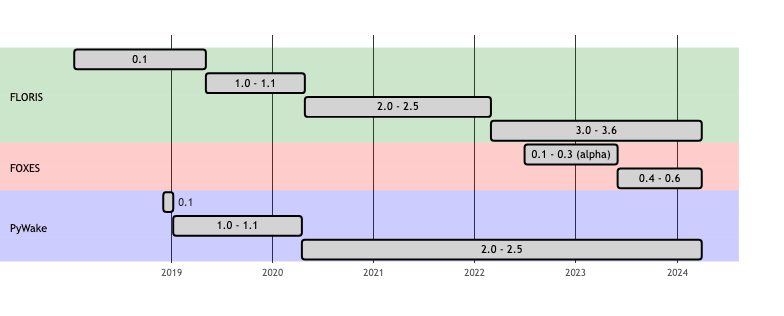
\includegraphics[width=0.9\textwidth]{model_timelines.png}
  % \vspace{-0.3cm}
  \caption{Release timeline for FLORIS, FOXES, and PyWake obtained from their respective source code repository release listings.}
  \label{fig:software_releases}
\end{figure}

\begin{table}[!hb]
\caption{The list of mathematical wind turbine wake velocity and deflection models, noted by ``$\bullet$'', available in each software project included in this study. The models common to at least two software, noted in bold, are compared in Section ~\ref{comparison}.}
\label{tab:models}
\centering
\begin{tabular}{llll}
\toprule
{Wake Velocity Model} & {FLORIS} & {FOXES} & {PyWake} \\ \midrule
\textbf{Jensen 1983}\cite{jensen1983note}                               & $\bullet$ & $\bullet$ & $\bullet$  \\
Larsen 2009\cite{larsen2009simple}                                      &           &           & $\bullet$  \\
\textbf{Bastankhah / Porté-Agel 2014}\cite{bastankhah2014new}           &           & $\bullet$ & $\bullet$  \\
\textbf{Bastankhah / Porté-Agel 2016}\cite{bastankhah2016experimental}  & $\bullet$ & $\bullet$ &            \\
Niayifar / Porté-Agel 2016\cite{niayifar2016analytical}                 &           &           & $\bullet$  \\
IEA Task37 Bastankhah 2018\cite{iea2018wake}                            &           &           & $\bullet$  \\
Carbajo Fuertes / Markfort / Porté-Agel 2018\cite{fuertes2018wind}      &           &           & $\bullet$  \\
Blondel / Cathelain 2020\cite{blondel2020alternative}                   &           &           & $\bullet$  \\
Zong / Porté-Agel 2020\cite{zong2020momentum}                           &           &           & $\bullet$  \\
Cumulative Curl 2022\cite{bay2023addressing}                            & $\bullet$ &           &            \\
\textbf{TurbOPark (Nygaard 2022)}\cite{nygaard2020modelling}            & $\bullet$*& $\bullet$ & $\bullet$  \\
Empirical Gauss 2023                                                    & $\bullet$ &           &            \\
\midrule
{Wake Deflection Model}                                                 &           &           &            \\
\midrule
\textbf{Jímenez 2010}\cite{jimenez2010application}                      & $\bullet$ &           & $\bullet$  \\
\textbf{Bastankhah / Porté-Agel 2016}\cite{bastankhah2016experimental}  & $\bullet$ & $\bullet$ &            \\
Larsen et al 2020\cite{larsen2020yaw}                                   &           &           & $\bullet$  \\
Empirical Gauss 2023                                                    & $\bullet$ &           &            \\
\bottomrule
\end{tabular}
\end{table}

\ind{}FLORIS has been in development at NREL in various forms since 2014, and the current iteration began in 2017.
FLORIS is designed to support the development and implementation of new wake models, as well as wind farm energy yield calculation and wind farm layout and controls design.
The software architecture is designed with explicit interfaces where new models can be integrated into the existing framework.

\ind{}FOXES has been in development since 2022 at Fraunhofer IWES.
It is designed as a modular tool for modelling aspects of wind farm calculations allowing users to combine existing models and easily add new models.
FOXES directly integrates with optimization libraries that allow for any variable to be optimized.

\ind{}PyWake has been in development at DTU since 2018.
It is used to study the interaction between turbines within a wind farm and its influence on the farm’s flow field and power production.
It has a modular architecture providing predefined modelling blocks for calculating annual energy production.

\ind{}The objective of this work is to establish the methods for characterising the similarities and differences across this class of software.
Reference data from experiments, high-fidelity simulations, or literature are intentionally excluded.
The focus is specifically on establishing the ensemble of results across common mathematical wake model implementations and capturing software-specific design decisions, and there is no intention to assign or imply correctness to any software’s implementation of a model.
For an evaluation of the wake models themselves, readers are referred to \cite{porteagel2020wind} and the publications specific to each model.
Due to the complexity of each software project and the number of parameters available in each, it is envisioned that the current work is the beginning of an ongoing study to fully characterize the aggregate modelling capabilities within this class of software.
In Section ~\ref{methods}, this paper describes the methods and tools used to conduct the comparison of the models and algorithms in the software.
Section ~\ref{comparison} details the comparisons of the common wake models.
Section ~\ref{discussion} provides a brief analysis of the comparison results, and Section ~\ref{conclusion} summarizes the study and proposes future work.

\section{Methods} \label{methods}

This study considers the software as comprising two primary components: the mathematical formulation and the implementation in computer code, as shown in Figure ~\ref{fig:model_components}.
Approaching with the perspective of software testing, the “grey box testing” technique \cite{william2009software}, common in software engineering, is applied to individual components of the software projects.
The individual mathematical and computational models are isolated within the testing environment, and the relevant results from the test suite are compared across the included software.

\begin{figure}[!htb]
  \centering
  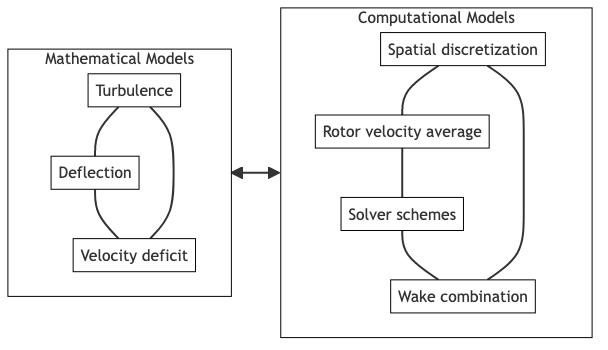
\includegraphics[width=0.6\textwidth]{figures/model_components.png}
  % \vspace{-0.3cm}
  \caption{ The primary components of the studied set of wake modelling software: mathematical models and their implementation as computational models.}
  \label{fig:model_components}
\end{figure}

\ind{}This study leverages the wake model comparison framework \textit{wcomp} \cite{wcomp01} to express the test cases and visualize the results.
\textit{wcomp} was made available by NREL in 2023, and it provides a common interface for Python-based wake modelling projects to interface to the \textit{windIO} ontology developed by the International Energy Agency Wind Technology Collaboration Programme (IEA Wind) Task 37 \cite{bortolotti2022system}, as shown in Figure ~\ref{fig:wcomp_arch}.

\begin{figure}[!htb]
  \centering
  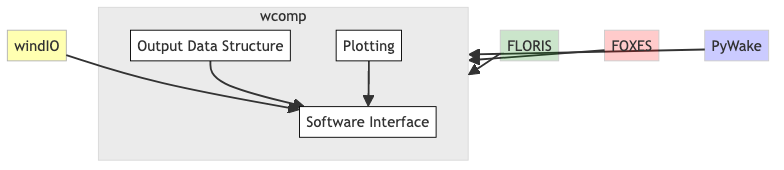
\includegraphics[width=0.6\textwidth]{figures/wcomp_architecture.png}
  % \vspace{-0.3cm}
  \caption{Architecture of the wake modelling software comparison framework \textit{wcomp} used to integrate the software compared in this study.}
  \label{fig:wcomp_arch}
\end{figure}

\ind{}The individual wake models are compared with two cases.
For all cases, the wind speed is 9.8 meters per second (m/s) at the hub height, turbulence intensity is 7.5\%, and air density is 1.225 kilograms per cubic meter (kg/m$^3$).
The turbine model is the IEA Wind Task 37 15-megawatt (MW) offshore reference turbine \cite{gaertner2020iea}, which has a rotor diameter (D) of 240 m and hub height of 150 m.
The first case has a single wind turbine oriented perpendicular to the incoming wind (no yaw misalignment).
The second case has four turbines placed in a line oriented with the incoming wind so that each turbine is directly behind the turbine upstream of it, and they are spaced at a distance of 5D (1200 m) apart.
For the deflection model comparison, the single turbine in the one-turbine case and the leading two turbines in the four-turbine case are yawed +10° (counter-clockwise if looking at the wind farm from above toward the ground).
Four one-dimension profiles are used to sample the x-component of the wind speed throughout the farm.
The turbine array layouts and one-dimensional profile locations are shown in Figure ~\ref{fig:case_setup} where:
\begin{itemize}
\item For all cases, a streamwise profile at hub height starts 1D upstream and extends 20D downstream of the last turbine,
\item For the one-turbine case, three lateral profiles extend 2D from the rotor center in each direction and are positioned at 1D, 5D, and 10D downstream.
\end{itemize}
Additionally, an absolute value of the difference between model implementation is included in each plot.

\begin{figure}[h]
\centering
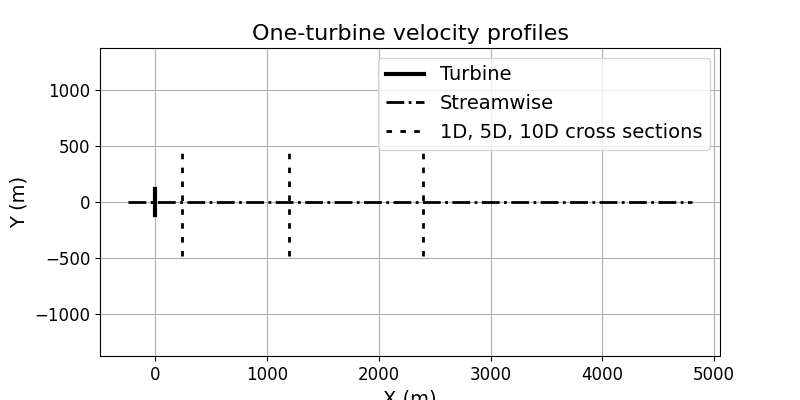
\includegraphics[width=0.35\textwidth]{figures/1t config.png}
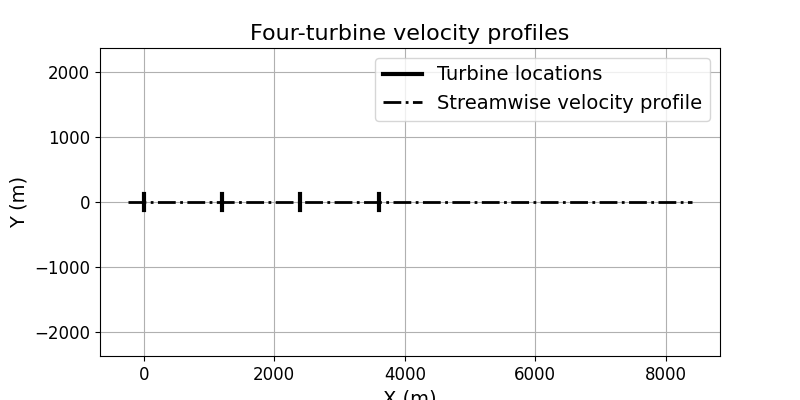
\includegraphics[width=0.35\textwidth]{figures/4t config.png}
\\
\caption{Turbine layout and one-dimension profile sample lines for one- and four-turbine cases.}
\label{fig:case_setup}
\end{figure}

\section{Mathematical wake model comparison} \label{comparison}

This section provides a comparison of the implementation of the mathematical wake models common to at least two of the three wake modelling software included in this study, as listed in Table ~\ref{tab:models}.
The mathematical wake model parameters are aligned across all the cases and are noted in the sections below.
However, additional computational model parameters are available as modeling decisions for the user.
Two notable parameters are the method to determine the average velocity across the rotor, used to compute the thrust coefficient, and the method to combine coincident wakes.
Because \textit{wcomp} and \textit{windIO} do not yet support the configuration of computational model parameters, they are left as the defaults to each software for this study.
Note that the difference between implementations of some models may be near zero making the difference line fall on the x-axis.

\subsection{Jensen 1983 wake velocity model}
The model proposed by NO Jensen in 1983 assumes a top-hat shape for the wake cross section.
The model is a function of the axial induction, rotor size, and distance downstream from the turbine producing the wake.
The only parameter for this model is the wake growth rate, \textit{k}, and it is set to 0.1.
FLORIS, FOXES, and PyWake implement this model, and all three are included in the comparison in Figure ~\ref{fig:jensen}.

\subsection{Bastankhah / Porté-Agel 2014 wake velocity model}
The Bastankhah / Porté-Agel 2014 model describes a self-similar Gaussian wake cross section.
Since it is valid only in the far-wake region, the calculation of the length of the near-wake is also included in the model.
It is a function of the thrust coefficient, rotor size, downstream distance and vertical and lateral distance from the turbine producing the wake.
The only parameter for this model is the wake growth rate, \textit{k*}, and it is set to 0.03.
This model is implemented in FOXES and PyWake, and their results are shown in Figure ~\ref{fig:b2014}.

\subsection{Bastankhah / Porté-Agel 2016 wake velocity model} \label{bastankhah_velocity}
The Bastankhah / Porté-Agel 2016 model is posed as model for the wake of a yawed wind turbine, and, for the sake of comparison, it is included here as a velocity model with wind turbines operating with no yaw misalignment.
In Section ~\ref{bastankhah_deflection}, it is compared again with wind turbine with yaw misalignment.
This model describes a self-similar Gaussian wake cross section similar to Bastankhah / Porté-Agel 2014.
It is also valid only in the far-wake region, so the calculation for the length of the near-wake region is included in the model.
It is a function of the wake-center deflection, thrust coefficient, rotor size, downstream distance, and vertical and lateral distance from the turbine producing the wake.
This model includes tuning parameters for the wake growth rate in the lateral and vertical directions, $k_{y}$ and $k_{z}$, respectively, and two parameters to influence the onset of the far-wake region, $\alpha$ and $\beta$.
The two wake growth rate parameters are set to equivalent values according to the empirical relationship proposed in \cite{niayifar2016analytical}, and $\alpha$ and $\beta$ are 0.58 and 0.077, respectively.
This model is implemented in FLORIS and FOXES, and their results are shown in Figure ~\ref{fig:b2016}.

\subsection{TurbOPark wake velocity model}
The Turbulence Optimized Park (TurbOPark) model was proposed in Nygaard 2022, and it consists of a wind turbine wake velocity model and a wind farm blockage model.
The velocity model is compared here, and the bloackage model is outside the scope of the current study.
The TurbOPark model builds on an earlier top-hat model to explicitly include effects of turbulence.
The wake growth rate, A, is set to 0.04.
This model is implemented in FLORIS, FOXES, and PyWake, but the FLORIS implementation of TurbOPark does not support calculating the velocity for points outside of the rotor swept area, so it cannot be compared.
The results for FOXES and PyWake are shown in Figure ~\ref{fig:turbopark}.

\begin{figure}[]
\centering
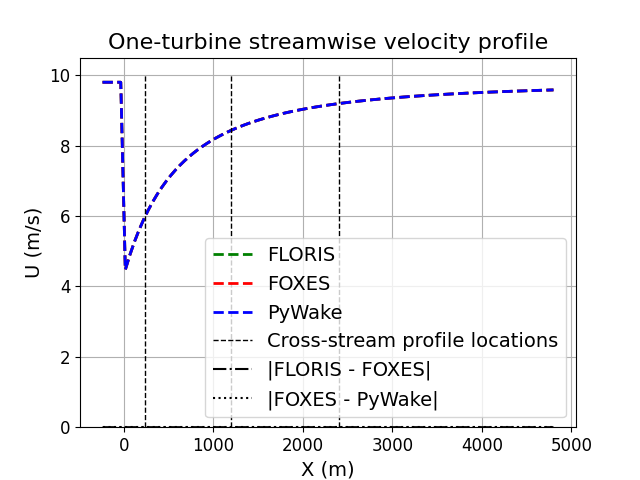
\includegraphics[width=0.35\textwidth]{figures/jensen 1t x.png}
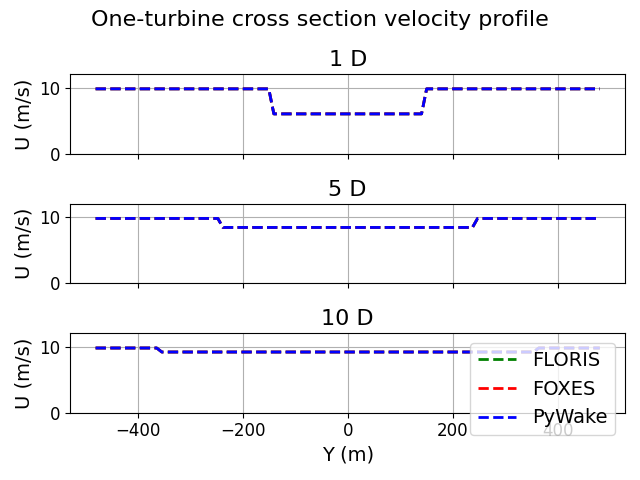
\includegraphics[width=0.35\textwidth]{figures/jensen 1t y.png}
\\
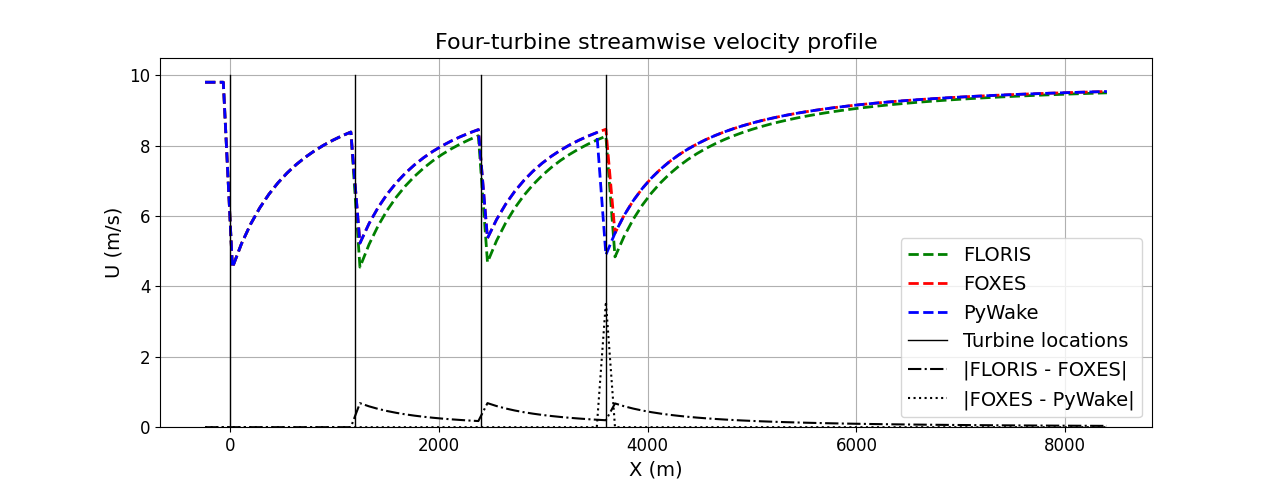
\includegraphics[width=0.7\textwidth]{figures/jensen 4t.png}
\caption{Jensen velocity model as implemented in FLORIS, FOXES, and PyWake compared with one-dimensional profiles in the streamwise and spanwise directions for a single turbine and a streamwise one-dimensional profile for a four-turbine array.}
\label{fig:jensen}
\end{figure}

\begin{figure}[]
\centering
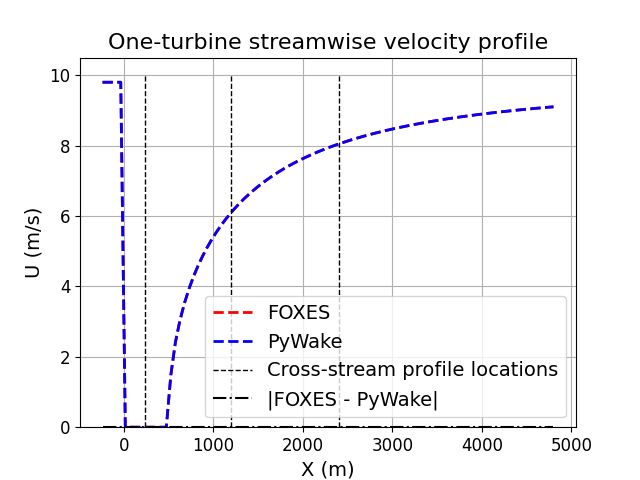
\includegraphics[width=0.35\textwidth]{figures/b2014 1t x.png}
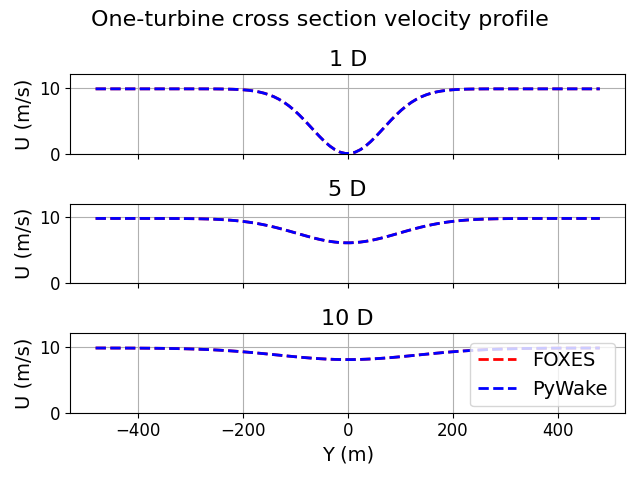
\includegraphics[width=0.35\textwidth]{figures/b2014 1t y.png}
\\
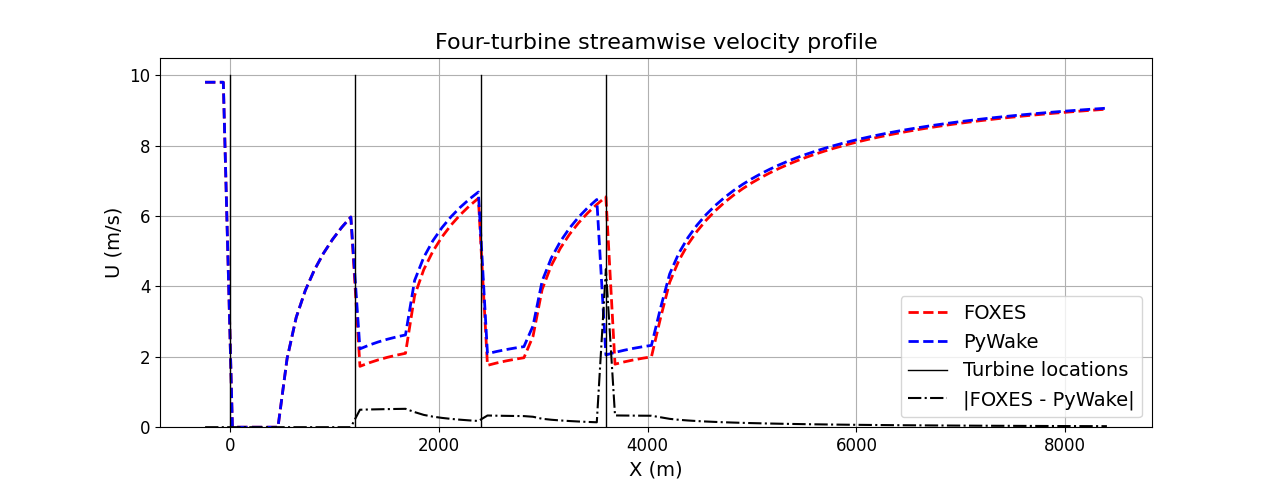
\includegraphics[width=0.7\textwidth]{figures/b2014 4t.png}
\caption{Bastankhah / Porté-Agel 2014 velocity model as implemented in FOXES and PyWake compared with one-dimensional profiles in the streamwise and spanwise directions for a single turbine and a streamwise one-dimensional profile for a four-turbine array.}
\label{fig:b2014}
\end{figure}

\begin{figure}[]
\centering
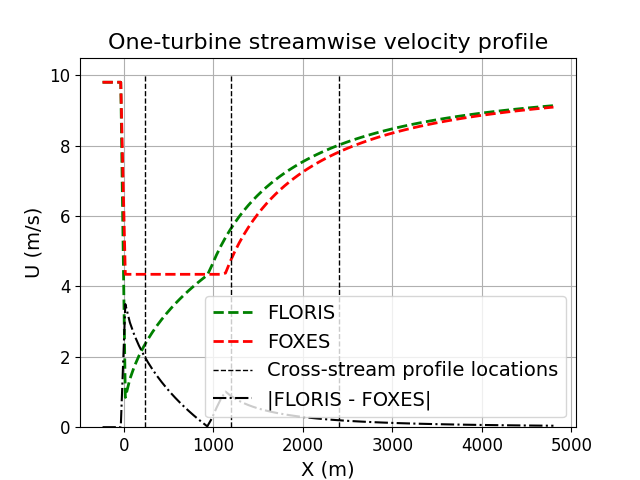
\includegraphics[width=0.35\textwidth]{figures/b2016 1t x.png}
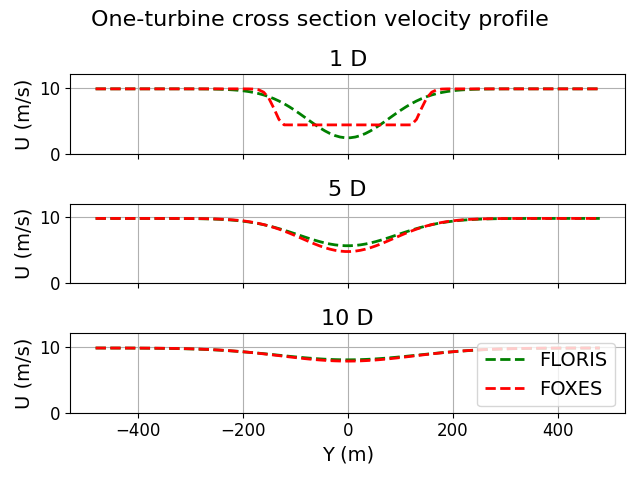
\includegraphics[width=0.35\textwidth]{figures/b2016 1t y.png}
\\
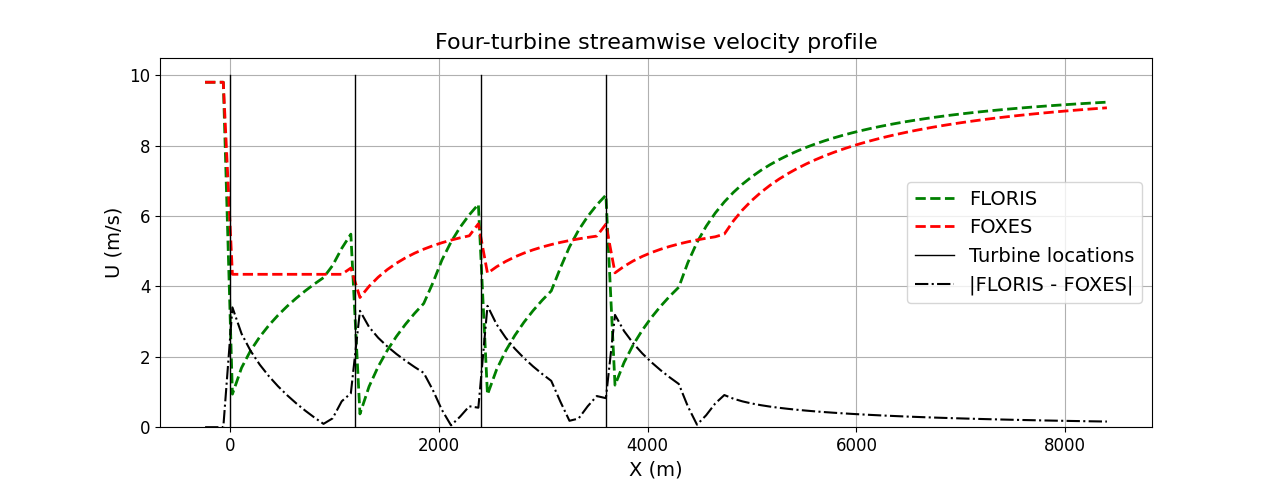
\includegraphics[width=0.7\textwidth]{figures/b2016 4t.png}
\caption{Bastankhah / Porté-Agel 2016 velocity model as implemented in FLORIS and FOXES compared with one-dimensional profiles in the streamwise and spanwise directions for a single turbine and a streamwise one-dimensional profile for a four-turbine array.}
\label{fig:b2016}
\end{figure}

\begin{figure}[]
\centering
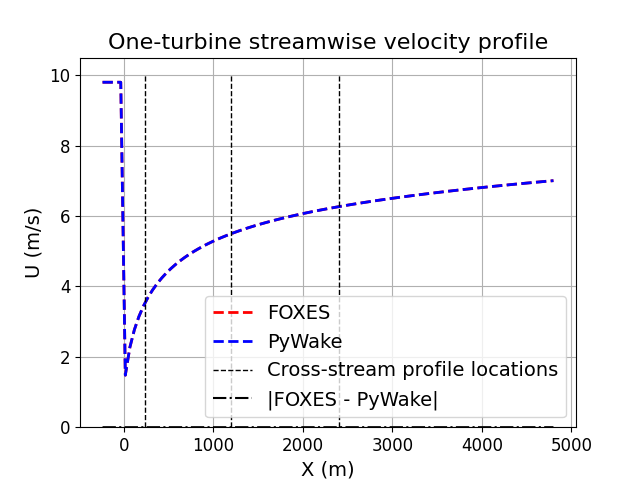
\includegraphics[width=0.35\textwidth]{figures/turbopark 1t x.png}
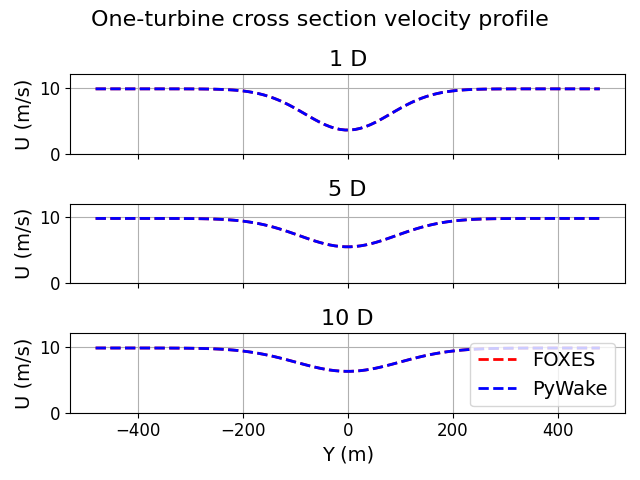
\includegraphics[width=0.35\textwidth]{figures/turbopark 1t y.png}
\\
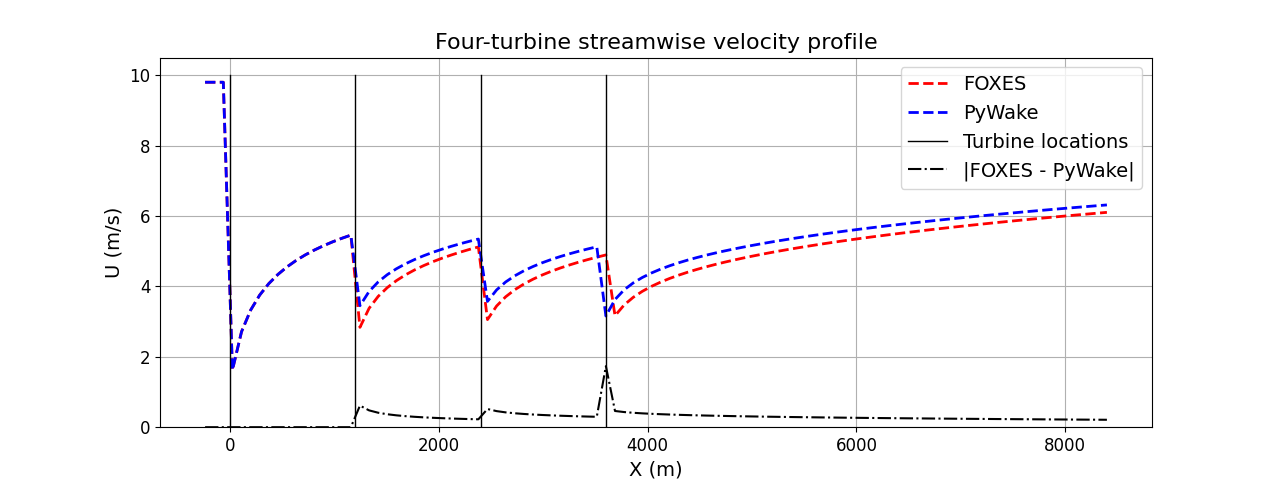
\includegraphics[width=0.7\textwidth]{figures/turbopark 4t.png}
\caption{TurbOPark velocity model as implemented in FOXES and PyWake compared with one-dimensional profiles in the streamwise and spanwise directions for a single turbine and a streamwise one-dimensional profile for a four-turbine array.}
\label{fig:turbopark}
\end{figure}

\subsection{Jímenez wake deflection model}
The Jímenez model for wake deflection assumes a top-hat shape for the wake cross section and calculates the wake skew angle from wake width, yaw angle, and thrust coefficient.
It includes a single parameter for the linear wake growth rate, $\beta$, and it is set to 0.1.
FLORIS and PyWake implement this model. Their results are shown in Figure ~\ref{fig:jimenez}.

\subsection{Bastankhah / Porté-Agel 2016  wake deflection model} \label{bastankhah_deflection}
The Bastankhah / Porté-Agel 2016 model proposes the velocity profile for the wake behind a yawed wind turbine.
See Section ~\ref{bastankhah_velocity} for additional information. This model is implemented in FLORIS and FOXES, and their results are shown in Figure ~\ref{fig:b2016_deflection}.

\begin{figure}[]
\centering
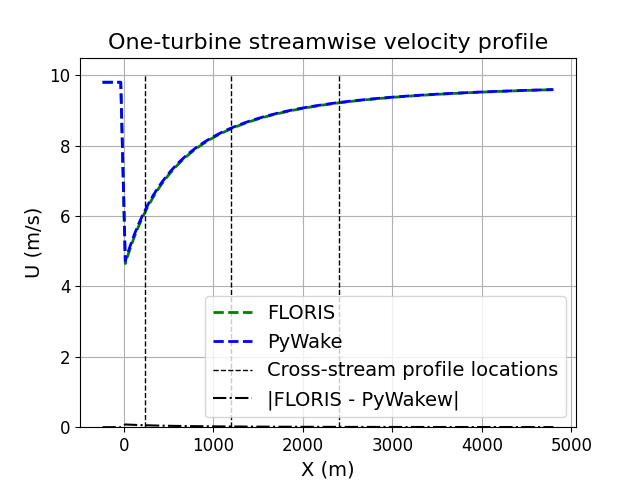
\includegraphics[width=0.35\textwidth]{figures/jimenez 1t x.png}
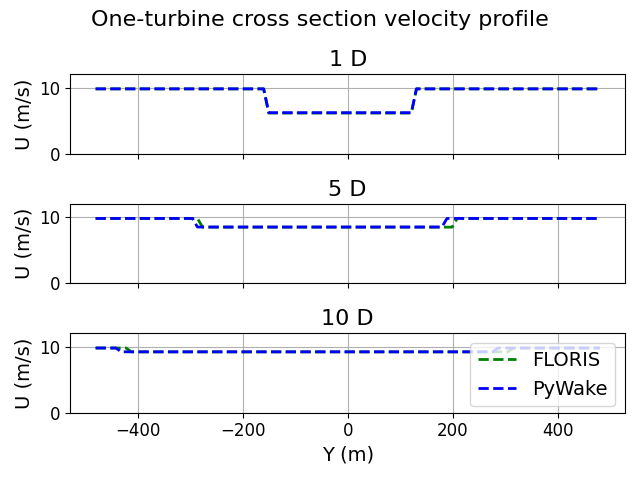
\includegraphics[width=0.35\textwidth]{figures/jimenez 1t y.png}
\\
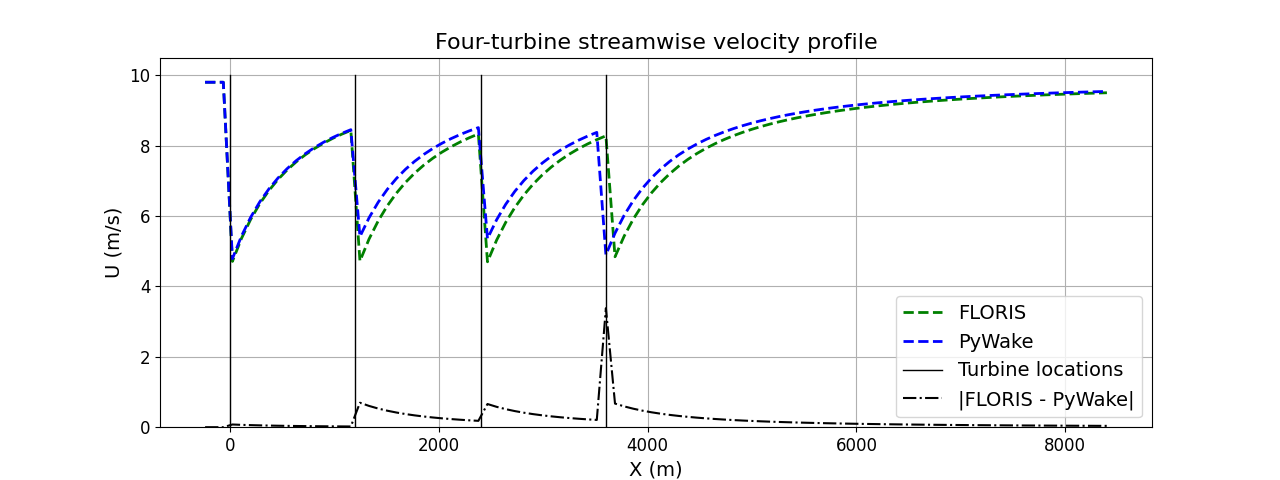
\includegraphics[width=0.7\textwidth]{figures/jimenez 4t.png}
\caption{Jímenez wake deflection model as implemented in FLORIS and PyWake compared with one-dimensional profiles in the streamwise and spanwise directions for a single turbine and a streamwise one-dimensional profile for a four-turbine array.
The single turbine and two leading turbines in the one- and four-turbine arrays, respectively, are yawed +10°}
\label{fig:jimenez}
\end{figure}

\begin{figure}[]
\centering
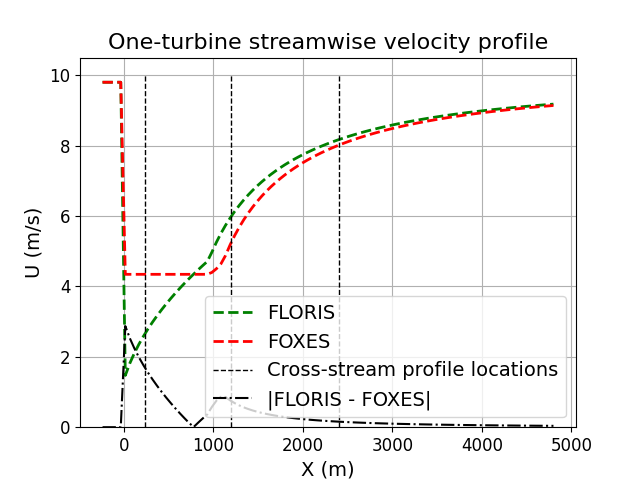
\includegraphics[width=0.35\textwidth]{figures/b2016 deflection 1t x.png}
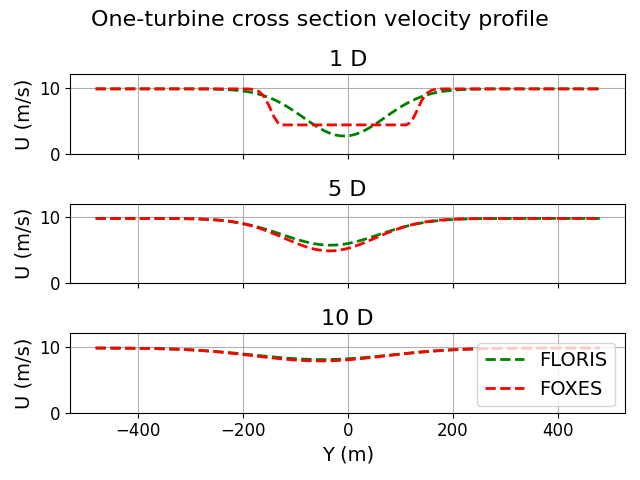
\includegraphics[width=0.35\textwidth]{figures/b2016 deflection 1t y.png}
\\
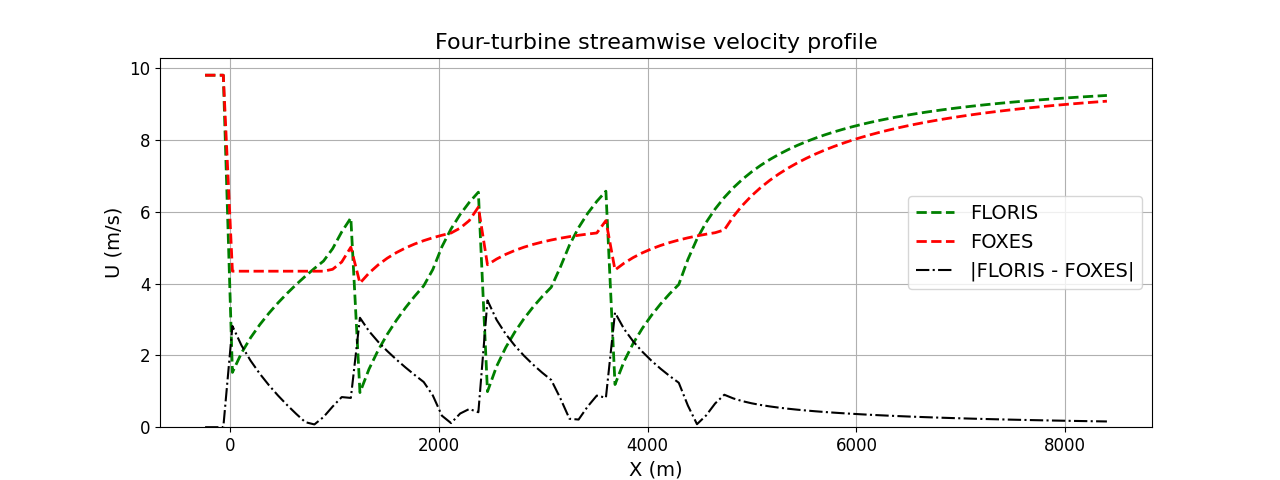
\includegraphics[width=0.7\textwidth]{figures/b2016 deflection 4t.png}
\caption{Bastankhah / Porté-Agel 2016 wake deflection model as implemented in FLORIS and FOXES compared with 1-dimensional profiles in the streamwise and spanwise directions for a single turbine and a streamwise one-dimensional profile for a four-turbine array.
The single turbine and two leading turbines in the one- and four-turbine arrays, respectively, are yawed +10°}
\label{fig:b2016_deflection}
\end{figure}

\section{Discussion} \label{discussion}

The L2-Norm of the differences between implementations of common models is listed in Table ~\ref{tab:error}, as measured by the one-dimensional streamwise profiles.
The agreement between software implementations is very high for the top-hat models: Jensen, TurbOPark, and Jímenez.
However, the Gaussian models from Bastankhah and Porté-Agel are less aligned.

\begin{table}[!h]
\caption{The L2 norm of the difference between mathematical wake models, where implemented (indicated by a $\bullet$). The Jensen model includes FLORIS-FOXES and FOXES-PyWake norms.}
\label{tab:error}
\centering
\begin{tabular}{llllll}
\toprule
{Wake Velocity Model} & {FLORIS} & {FOXES} & {PyWake} & {One-Turbine L2 Norm}& {Four-Turbine L2 Norm}\\ \midrule
Jensen 1983                            & $\bullet$ & $\bullet$ & $\bullet$ & 0.00, 0.00 & 2.63, 3.56 \\
Bastankhah / Porté-Agel 2014           &           & $\bullet$ & $\bullet$ & 0.00 & 4.92 \\
Bastankhah / Porté-Agel 2016           & $\bullet$ & $\bullet$ &           & 7.70 & 13.01\\
TurbOPark (Nygaard 2022)               & $\bullet$*& $\bullet$ & $\bullet$ & 0.00 & 3.31 \\
\midrule
{Wake Deflection Model}                &           &           &           &      &      \\
\midrule
Jímenez 2010                           & $\bullet$ &           & $\bullet$ & 0.22 & 4.27\\
Bastankhah / Porté-Agel 2016           & $\bullet$ & $\bullet$ & $\bullet$ & 6.44 & 12.37\\
\bottomrule
\end{tabular}
\end{table}

\ind{}The Gaussian models included in this study are only valid in the far-wake region, and the calculation for the beginning of that region is a part of the model.
From Figure ~\ref{fig:b2016} for the Bastankhah / Porté-Agel 2016 model, it is seen that the FOXES implementation calculates the near-wake to far-wake transition point at approximately 5 rotor diameters downstream, whereas the FLORIS transition occurs at approximately 4.5 rotor diameters downstream.
The differences between the model implementations reduces as the wake continues to recover after the last turbine indicating that the differences in solutions would have the most impact in dense wind farm layouts.
Another difference between the FLORIS and FOXES implementations on this model is the near-wake treatment.
Figure ~\ref{fig:b2016} shows that FOXES models the near-wake with a constant velocity while FLORIS models a ramp up from the initial velocity deficit to the far-wake deficit.

\ind{}The difference norms for the one-turbine cases are significantly lower than for the four-turbine cases.
From Figures ~\ref{fig:jensen}, ~\ref{fig:b2014}, ~\ref{fig:turbopark}, and ~\ref{fig:jimenez}, it is clear that the difference is a function of the depth within a wind turbine array.
This difference in the calculated results is likely due to the default methods for calculating the rotor average wind speed, modeling axial induction, and treatment of turbulence intensity induced by the turbine itself.

\section{Conclusion} \label{conclusion}

This work brings together three open-source research software projects from the wind farm wake modeling community to identify and characterize the ensemble of results for mathematical wake models that they implement in common.
FLORIS from the National Renewable Energy Laboratory, FOXES from Fraunhofer Institute for Wind Energy Systems, and PyWake from the Technical University of Denmark are each integrated into a central framework, \textit{wcomp}, that provides an interface to a common wind energy system ontology, \textit{windIO}.

\ind{}By providing a common ontology and the mechanisms to extract results in a consistent manner, implementations of mathematical wake models across software projects are directly compared.
Overall, the wake model implementations are generally in agreement across the software, but implementation details are evident in the results.
In order to accurately identify the root cause of the differences across the software, additional modeling considerations should be aligned, such as the method to average the wind speed across the rotor, grid point location and density, wind shear modeling, wake combination methods, turbulence intensity modeling, and handling for partially waked wind turbines.

\ind{}This study presents the initial framework for what the authors intend to be a regular component of the wind turbine wake modeling research community.
Future work in this area will include close collaborations between the developers of each software project to add additional parameterized studies, and the \textit{wcomp} framework and \textit{windIO} ontology will be expanded to enable configuring computational model parameters and other implementation details.
Finally, the methods and results are anticipated to be presented in an online, open-source dashboard where the wind farm wake modeling community can submit new cases for comparison across the included projects and new project teams can register their software to be included in the comparisons.

\section{Code Availability}
Interested readers can recreate this study by installing \textit{wcomp}; see https://rafmudaf.github.io/wcomp/.
All of the figures included here are taken directly from the following Jupyter Notebooks:

\begin{itemize}
\item \texttt{https://github.com/rafmudaf/wcomp/blob/main/examples/torque2024\_1turbine.ipynb}

\item \texttt{https://github.com/rafmudaf/wcomp/blob/main/examples/torque2024\_4turbine.ipynb}
\end{itemize}

\bibliography{bibliography.bib}

\end{document}
